\subsection{LIF Spike Response}

Let us discuss a more general case:

\begin{equation}
    v(t) + \tau_m \cdot \dot{v}(t) = I(t) \cdot \exp(\alpha \cdot t)
\end{equation}
    
A helpful definition will be: \(f(t) = \int I(t) \cdot dt + B\) \\
Our guess for a solution: \(v(t) = f(t) \cdot \exp(\alpha \cdot t)\) \\
The derivative: \(\dot{v}(t) = \alpha \cdot \exp(\alpha \cdot t) \cdot f(t) + \exp(\alpha \cdot t) \cdot \dot{f}(t)\)
    
\begin{equation}
    v(t) + \tau_m \cdot \dot{v}(t) = (1 + \alpha \cdot \tau_m) \cdot \exp(\alpha \cdot t) \cdot f(t) + \exp(\alpha \cdot t) \cdot \dot{f}(t)
\end{equation}
    
If \(1 + \alpha \cdot \tau_m = 0\) \(\implies\) \(v(t) + \tau_m \cdot \dot{v}(t) = \exp(\alpha \cdot t) \cdot \dot{f}(t) = I(t) \cdot \exp(\alpha \cdot t)\) \\


Why this solution is useful? \\
\(\delta(t)\) = Dirac delta function \\
\(H(t)\) = Heaviside function = \(\int \delta(t) \cdot dt\) \\
The refractory period will stay the same throughout  

\begin{equation}
	I(t) = I_0 \cdot \delta(t)
\end{equation}

It is easy to conclude the following: 

\begin{equation}
	I(t) = I_0 \cdot \delta(t) = I_0 \cdot \exp(-t/\tau_m) \cdot \delta(t)
\end{equation}
If we set 

\begin{equation}
	I(t) = I_0 \cdot \delta(t)
\end{equation}

According to 5.6:

\begin{equation}
	v(t) = (\int I(t) \cdot dt + B) \cdot \exp(-t/\tau_m)
\end{equation}

\begin{equation}
	v(t) = (I_0 \cdot H(t) + B) \cdot \exp(-t/\tau_m)
\end{equation}

For the condition: 

\begin{equation}
	v(t=0) = I_0
\end{equation}

\begin{equation}
	v(t) = I_0 \cdot H(t) \cdot \exp(-t/\tau_m)
\end{equation}

By linearity of the integration, we conclude the following:
For the input:

\begin{equation}
	I(t) = \sum_i I_0 \cdot \delta(t-t_i) \quad \text{s.t.} \quad \{t_i\}_i = \text{input firing times}
\end{equation}

Our result will be:
\begin{equation}
	v(t) = \sum_i I_0 \cdot H(t-t_i) \cdot \exp(-(t-t_i)/\tau_m)
\end{equation}

And as we can see once we add the refractory period into consideration:

\begin{figure}[H]
    \centering
    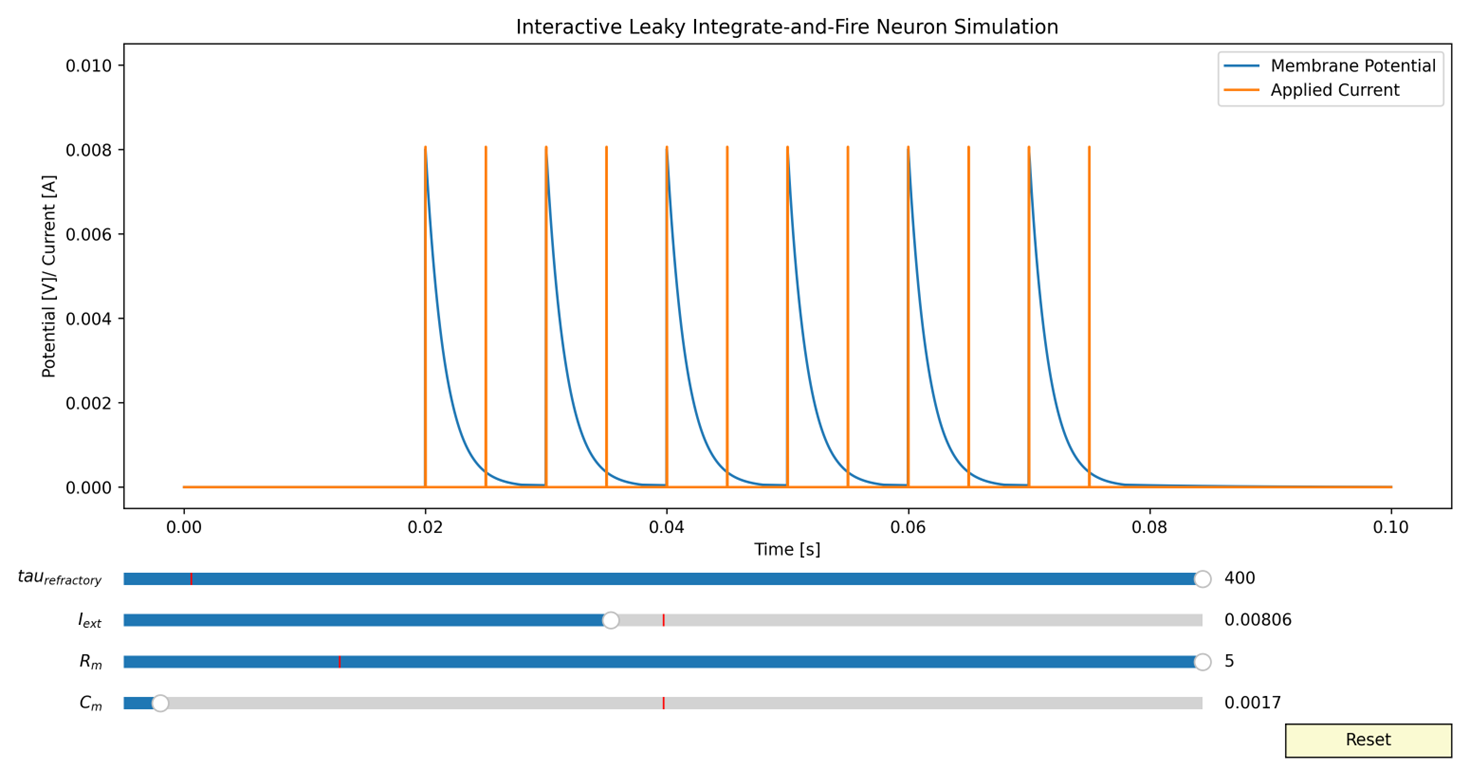
\includegraphics[width=0.8\textwidth]{methods/computational-models/graphs/LIF-spike-response-ref.png}
    \caption{LIF membrane voltage response to delta train input current}
    \label{fig:LIF-spike-ref}
\end{figure}

(*) for the above graph: \( I_0=V_{\text:thresh} \implies \) every input spike will cause the neuron to reach its action potential.

To demonstrate the sum of reactions of the given input:

\begin{figure}[H]
    \centering
    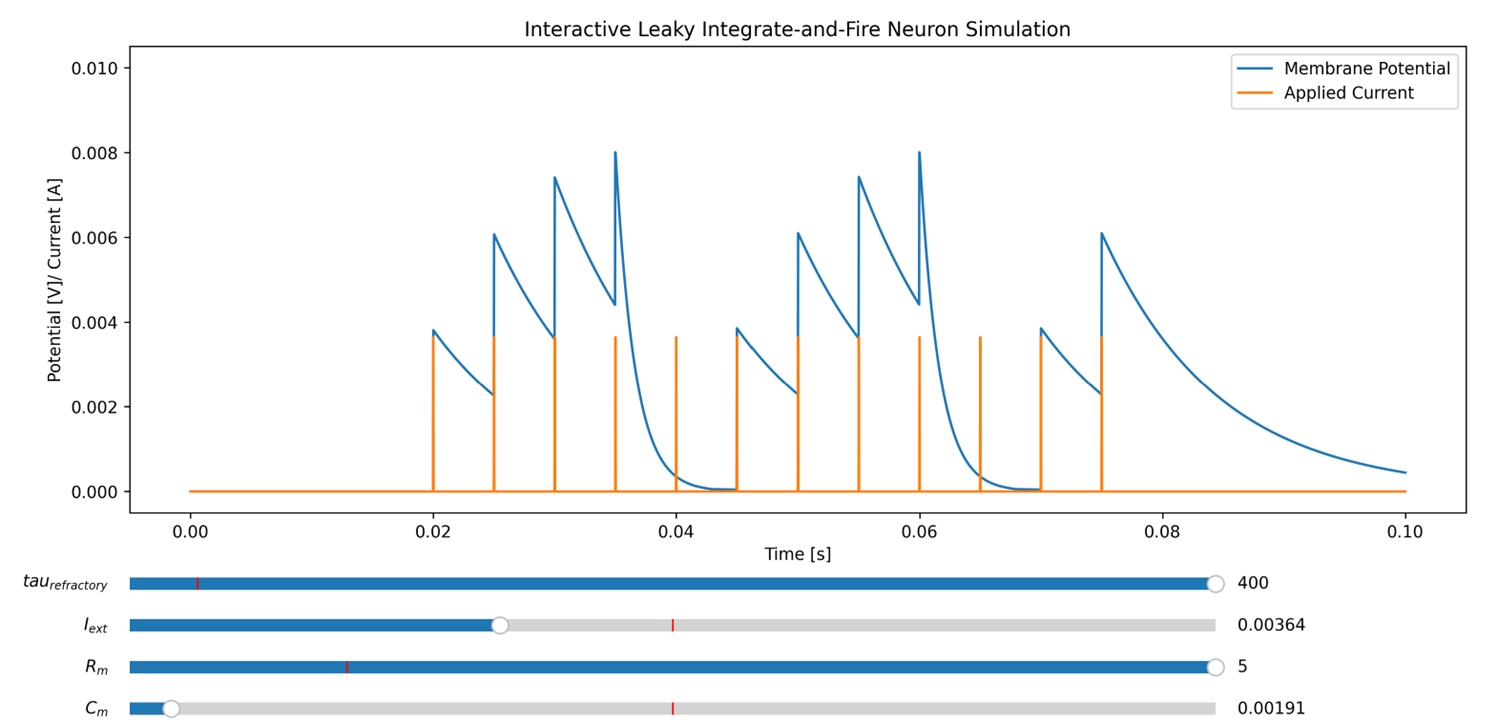
\includegraphics[width=0.8\textwidth]{methods/computational-models/graphs/LIF-high-freq-spike-response-ref.png}
    \caption{LIF membrane voltage response to high frequency delta train input current}
    \label{fig:LIF-high-freq-spike-ref}
\end{figure}

As we can see, when \(I_0 < V_{\text{thresh}}\), the voltage “spikes” for every \(I_0 \cdot \delta(t-t_i)\) till reaching the action potential and drops between input spikes. 

Let us take this a step further and find the firing frequency \(f(I_0, T)\) for a periodic delta train function:
\begin{equation}
I(t) = I_0 \cdot \sum_{n=0}^N \delta(t-n \cdot T)
\end{equation}
where \(T\) is the constant time period of the function and \(f = \frac{1}{T}\) is the frequency of the function.

For simplicity measures, we will assume: \(\tau_{\text{ref}} = 0\) and \(v_{\text{reset}} = 0\).
From the previous equation (7.1), we can conclude that the output for such an input will be:
\begin{equation}
v(t) = I_0 \cdot \sum_{n=0}^N H(t-n \cdot T) \cdot e^{-((t-n \cdot T)/\tau_m)}
\end{equation}

If \(v_{\text{th}} \leq I_0 \cdot \sum_{n=0}^{n_0} e^{-n \cdot T/\tau_m}\), then \(f(I_0, T) \geq \frac{1}{n_0} \cdot f\)

And if \(v_{\text{th}} \geq I_0 \cdot \sum_{n=0}^{n_0} e^{-n \cdot T/\tau_m}\), then \(f(I_0, T) \leq \frac{1}{n_0} \cdot f\)

Overall, we got:
\begin{equation}
f(I_0, T) = \frac{1}{n_0} \cdot f \quad \text{s.t.} \quad \sum_{n=0}^{n_0} e^{-n \cdot T/\tau_m} \leq v_{\text{th}} < I_0 \cdot \sum_{n=0}^{n_0+1} e^{-n \cdot T/\tau_m}
\end{equation}

The following graph will demonstrate the relation between \(f\), \(I_0\), and the firing frequency \(f(T, I_0)\):

\begin{figure}[H]
    \centering
    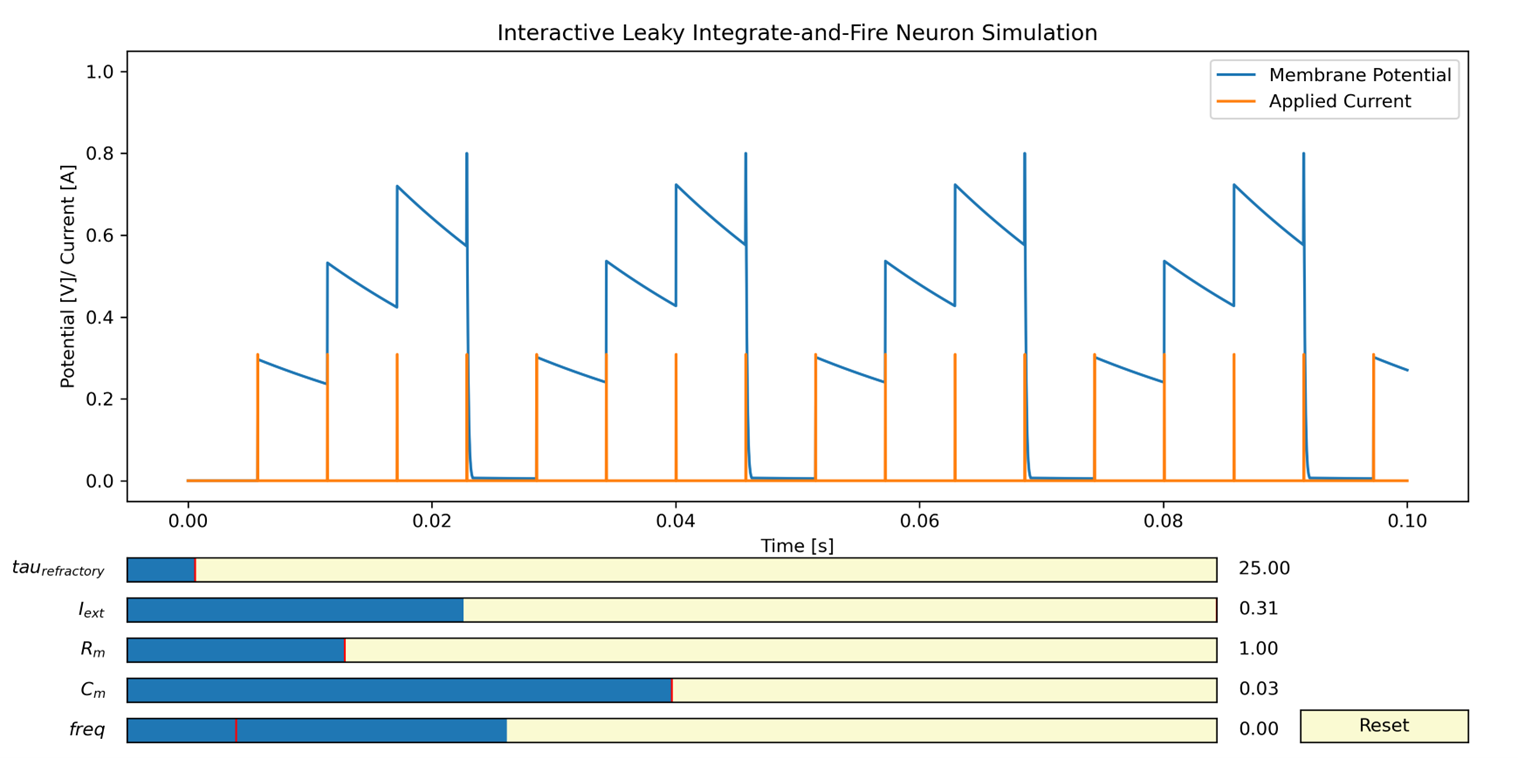
\includegraphics[width=0.8\textwidth]{methods/computational-models/graphs/LIF-high-freq-spike-response-ref-final.png}
    \caption{LIF membrane voltage response to high frequency delta spike trains with refractory period}
    \label{fig:LIF-high-freq-spike-ref-final}
\end{figure}
